% DW-TAL Decoupled Assignment Diagram (English — relative positioning, zero overlap)
\documentclass[tikz,border=3pt]{standalone}
\usepackage{fontspec}
\usepackage{amsmath,amssymb}
\setmainfont{DejaVu Serif}
\usetikzlibrary{positioning,fit,calc,arrows.meta,backgrounds}

\definecolor{cInk}{HTML}{1F2937}
\definecolor{cIn}{HTML}{F1F5F9}
\definecolor{cSel}{HTML}{E0F2FE}
\definecolor{cSelB}{HTML}{0369A1}
\definecolor{cCal}{HTML}{D1FAE5}
\definecolor{cCalB}{HTML}{047857}
\definecolor{cWarn}{HTML}{FEE2E2}
\definecolor{cWarnB}{HTML}{B91C1C}

\begin{document}
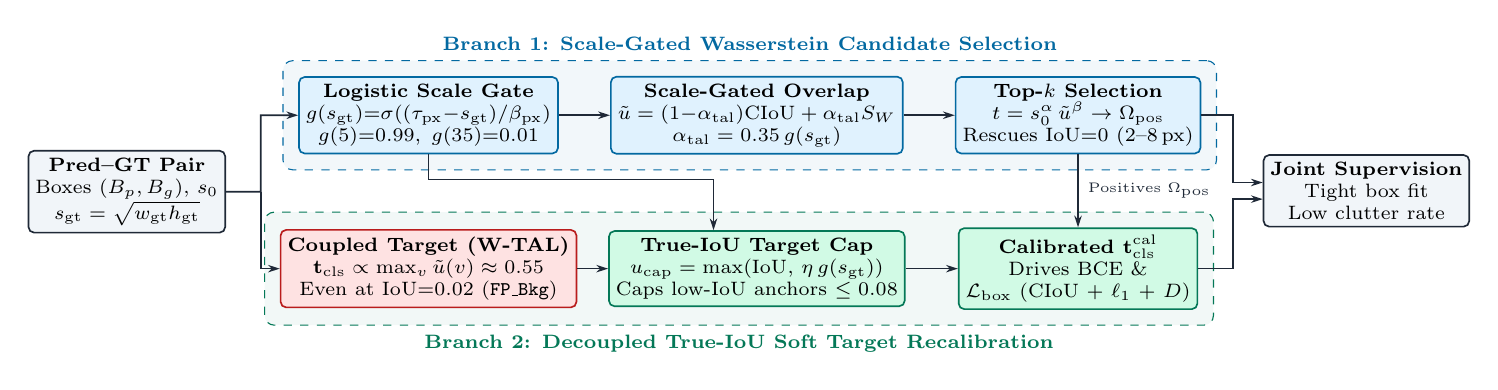
\begin{tikzpicture}[
  font=\scriptsize,
  blk/.style={draw=cInk, fill=#1, semithick, rounded corners=2pt,
              align=center, inner sep=2.5pt, minimum height=7.2mm},
  arr/.style={-{Stealth[length=1.5mm,width=0.95mm]}, cInk, semithick},
  zone/.style={draw=#1, dashed, rounded corners=3.5pt, fill=#1!5!white, inner sep=5.5pt},
]

\node[blk=cSel, draw=cSelB, minimum width=2.95cm] (gate)
  {\textbf{Logistic Scale Gate}\\$g(s_{\mathrm{gt}}){=}\sigma((\tau_{\mathrm{px}}{-}s_{\mathrm{gt}})/\beta_{\mathrm{px}})$\\$g(5){=}0.99,\; g(35){=}0.01$};
\node[blk=cSel, draw=cSelB, minimum width=3.15cm, right=0.65cm of gate] (blend)
  {\textbf{Scale-Gated Overlap}\\$\tilde{u} = (1{-}\alpha_{\mathrm{tal}})\mathrm{CIoU} + \alpha_{\mathrm{tal}} S_W$\\$\alpha_{\mathrm{tal}} = 0.35\,g(s_{\mathrm{gt}})$};
\node[blk=cSel, draw=cSelB, minimum width=2.85cm, right=0.65cm of blend] (topk)
  {\textbf{Top-$k$ Selection}\\$t = s_0^\alpha\,\tilde{u}^\beta \to \Omega_{\mathrm{pos}}$\\Rescues $\mathrm{IoU}{=}0$ ($2\text{--}8$\,px)};

\node[blk=cWarn, draw=cWarnB, minimum width=2.95cm, below=0.95cm of gate] (rawt)
  {\textbf{Coupled Target (W-TAL)}\\$\mathbf{t}_{\mathrm{cls}} \propto \max_v \tilde{u}(v) \approx 0.55$\\Even at $\mathrm{IoU}{=}0.02$ (\texttt{FP\_Bkg})};
\node[blk=cCal, draw=cCalB, minimum width=3.15cm] at (blend |- rawt) (cap)
  {\textbf{True-IoU Target Cap}\\$u_{\mathrm{cap}}=\max(\mathrm{IoU},\, \eta\,g(s_{\mathrm{gt}}))$\\Caps low-IoU anchors $\le 0.08$};
\node[blk=cCal, draw=cCalB, minimum width=2.85cm] at (topk |- rawt) (cal)
  {\textbf{Calibrated $\mathbf{t}_{\mathrm{cls}}^{\mathrm{cal}}$}\\Drives BCE \&\\$\mathcal{L}_{\mathrm{box}}$ (CIoU + $\ell_1$ + $D$)};

\coordinate (midL) at ($(gate.south west)!0.5!(rawt.north west)$);
\node[blk=cIn, minimum width=2.35cm, left=0.80cm of midL] (inp)
  {\textbf{Pred--GT Pair}\\Boxes $(B_p, B_g)$, $s_0$\\$s_{\mathrm{gt}}=\sqrt{w_{\mathrm{gt}}h_{\mathrm{gt}}}$};

\coordinate (midR) at ($(topk.south east)!0.5!(cal.north east)$);
\node[blk=cIn, minimum width=2.25cm, right=0.80cm of midR] (lossout)
  {\textbf{Joint Supervision}\\Tight box fit\\Low clutter rate};

\coordinate (splitL) at ($(inp.east)!0.48!(gate.west |- inp.east)$);
\draw[arr] (inp.east) -- (splitL) |- (gate.west);
\draw[arr] (splitL) |- (rawt.west);

\draw[arr] (gate.east) -- (blend.west);
\draw[arr] (blend.east) -- (topk.west);
\draw[arr] (rawt.east) -- (cap.west);
\draw[arr] (cap.east) -- (cal.west);

\draw[arr] (topk.south) -- node[right, font=\tiny]{Positives $\Omega_{\mathrm{pos}}$} (cal.north);
\draw[arr] (gate.south) -- ++(0,-0.32cm) -| ([xshift=-0.55cm]cap.north);

\coordinate (joinR) at ($(topk.east)!0.52!(lossout.west |- topk.east)$);
\draw[arr] (topk.east) -- (joinR) |- ([yshift=3pt]lossout.west);
\draw[arr] (cal.east) -- (topk.east |- cal.east) -- (joinR |- cal.east) |- ([yshift=-3pt]lossout.west);

\begin{scope}[on background layer]
  \node[zone=cSelB, fit=(gate)(blend)(topk), label={[font=\scriptsize\bfseries, text=cSelB]above:{Branch 1: Scale-Gated Wasserstein Candidate Selection}}] {};
  \node[zone=cCalB, fit=(rawt)(cap)(cal), label={[font=\scriptsize\bfseries, text=cCalB]below:{Branch 2: Decoupled True-IoU Soft Target Recalibration}}] {};
\end{scope}

\end{tikzpicture}
\end{document}
